
%\begin{document}

\section{\color{olive}Excercise 4}

\begin{figure}[!] %cambie la H por un !
\begin{centering}
\begin{tabular}{|c|c|c|c|c|c|c|c|}
\hline
$x_{1}$  & $x_{2}$  & $x_{3}$  & $x_{4}$  & $f_{1}$  & $f_{2}$  & $f_{3}$  & $f_{4}$\tabularnewline
\hline
\hline
0  & 0  & 0  & 0  & 0  & 0  & 0  & 0\tabularnewline
\hline
0  & 0  & 0  & 1  & 1  & 1  & 1  & 1\tabularnewline
\hline
0  & 0  & 1  & 0  & 1  & 1  & 1  & 0\tabularnewline
\hline
0  & 0  & 1  & 1  & 1  & 1  & 0  & 1\tabularnewline
\hline
0  & 1  & 0  & 0  & 1  & 1  & 0  & 0\tabularnewline
\hline
0  & 1  & 0  & 1  & 1  & 0  & 1  & 1\tabularnewline
\hline
0  & 1  & 1  & 0  & 1  & 0  & 1  & 0\tabularnewline
\hline
0  & 1  & 1  & 1  & 1  & 0  & 0  & 1\tabularnewline
\hline
1  & 0  & 0  & 0  & 1  & 0  & 0  & 0\tabularnewline
\hline
1  & 0  & 0  & 1  & 0  & 1  & 1  & 1\tabularnewline
\hline
1  & 0  & 1  & 0  & 0  & 1  & 1  & 0\tabularnewline
\hline
1  & 0  & 1  & 1  & 0  & 1  & 0  & 1\tabularnewline
\hline
1  & 1  & 0  & 0  & 0  & 1  & 0  & 0\tabularnewline
\hline
1  & 1  & 0  & 1  & 0  & 0  & 1  & 1\tabularnewline
\hline
1  & 1  & 1  & 0  & 0  & 0  & 1  & 0\tabularnewline
\hline
1  & 1  & 1  & 1  & 0  & 0  & 0  & 1\tabularnewline
\hline
\end{tabular}
\par\end{centering}
\caption{\color{cyan}Two's Complement truth table for 4 bits}
\end{figure}

If we write every signle input bit according to the minterms, we get the following equations:
\begin{center}
$f_{1}(m_{i})=m_{1}+m_{2}+m_{3}+m_{4}+m_{5}+m_{6}+m_{7}+m_{8}$
\par\end{center}

\begin{center}
$f_{2}(m_{i})=m_{1}+m_{2}+m_{3}+m_{4}+m_{9}+m_{10}+m_{11}+m_{12}$
\par\end{center}

\begin{center}
$f_{3}(m_{i})=m_{1}+m_{2}+m_{5}+m_{6}+m_{9}+m_{10}+m_{13}+m_{14}$
\par\end{center}

\begin{center}
$f_{4}(m_{i})=m_{1}+m_{3}+m_{5}+m_{7}+m_{9}+m_{11}+m_{13}+m_{15}$
\par\end{center}

Replacing the values of each minterm, we get the following:
\begin{center}
$f_{1}(x_{1};x_{2};x_{3};x_{4})=\bar{x_{1}}\bar{x_{2}}\bar{x_{3}}x_{4}+\bar{x_{1}}\bar{x_{2}}x_{3}\bar{x_{4}}+\bar{x_{1}}\bar{x_{2}}x_{3}x_{4}+\bar{x_{1}}x_{2}\bar{x_{3}}\bar{x_{4}}+\bar{x_{1}}x_{2}\bar{x_{3}}x_{4}+\bar{x_{1}}x_{2}x_{3}\bar{x_{4}}+\bar{x_{1}}x_{2}x_{3}x_{4}+x_{1}\bar{x_{2}}\bar{x_{3}}\bar{x_{4}}$
\par\end{center}

\begin{center}
$f_{2}(x_{1};x_{2};x_{3};x_{4})=\bar{x_{1}}\bar{x_{2}}\bar{x_{3}}x_{4}+\bar{x_{1}}\bar{x_{2}}x_{3}\bar{x_{4}}+\bar{x_{1}}\bar{x_{2}}x_{3}x_{4}+\bar{x_{1}}x_{2}\bar{x_{3}}\bar{x_{4}}+x_{1}\bar{x_{2}}\bar{x_{3}}x_{4}+x_{1}\bar{x_{2}}x_{3}\bar{x_{4}}+x_{1}\bar{x_{2}}x_{3}x_{4}+x_{1}x_{2}\bar{x_{3}}\bar{x_{4}}$
\par\end{center}

\begin{center}
$f_{3}(x_{1};x_{2};x_{3};x_{4})=\bar{x_{1}}\bar{x_{2}}\bar{x_{3}}x_{4}+\bar{x_{1}}\bar{x_{2}}x_{3}\bar{x_{4}}+\bar{x_{1}}x_{2}\bar{x_{3}}x_{4}+\bar{x_{1}}x_{2}x_{3}\bar{x_{4}}+x_{1}\bar{x_{2}}\bar{x_{3}}x_{4}+x_{1}\bar{x_{2}}x_{3}\bar{x_{4}}+x_{1}x_{2}\bar{x_{3}}x_{4}+x_{1}x_{2}x_{3}\bar{x_{4}}$
\par\end{center}

\begin{center}
$f_{4}(x_{1};x_{2};x_{3};x_{4})=\bar{x_{1}}\bar{x_{2}}\bar{x_{3}}x_{4}+\bar{x_{1}}\bar{x_{2}}x_{3}x_{4}+\bar{x_{1}}x_{2}\bar{x_{3}}x_{4}+\bar{x_{1}}x_{2}x_{3}x_{4}+x_{1}\bar{x_{2}}\bar{x_{3}}x_{4}+x_{1}\bar{x_{2}}x_{3}x_{4}+x_{1}x_{2}\bar{x_{3}}x_{4}+x_{1}x_{2}x_{3}x_{4}$
\par\end{center}

By simplification methods and properties, we can achieve this
four formulas to describe each output bit according to the input bits:
\begin{center}
$f_{1}(x_{1};x_{2};x_{3};x_{4})=x_{1}\bar{x_{2}}\bar{x_{3}}\bar{x_{4}}+\bar{x_{1}}(x_{2}+x_{3}+x_{4})$
\par\end{center}

\begin{center}
$f_{2}(x_{1};x_{2};x_{3};x_{4})=x_{2}\bar{x_{3}}\bar{x_{4}}+\bar{x_{2}}(x_{3}+x_{4})$
\par\end{center}

\begin{center}
$f_{3}(x_{1};x_{2};x_{3};x_{4})=x_{3}\bar{x_{4}}+\bar{x_{3}}x_{4}$
\par\end{center}

\begin{center}
$f_{4}(x_{1};x_{2};x_{3};x_{4})=x_{4}$
\par\end{center}

The previous formulas can be represented in logic gates' graphs:

\begin{figure}[!] %cambio la H por !
\begin{centering}
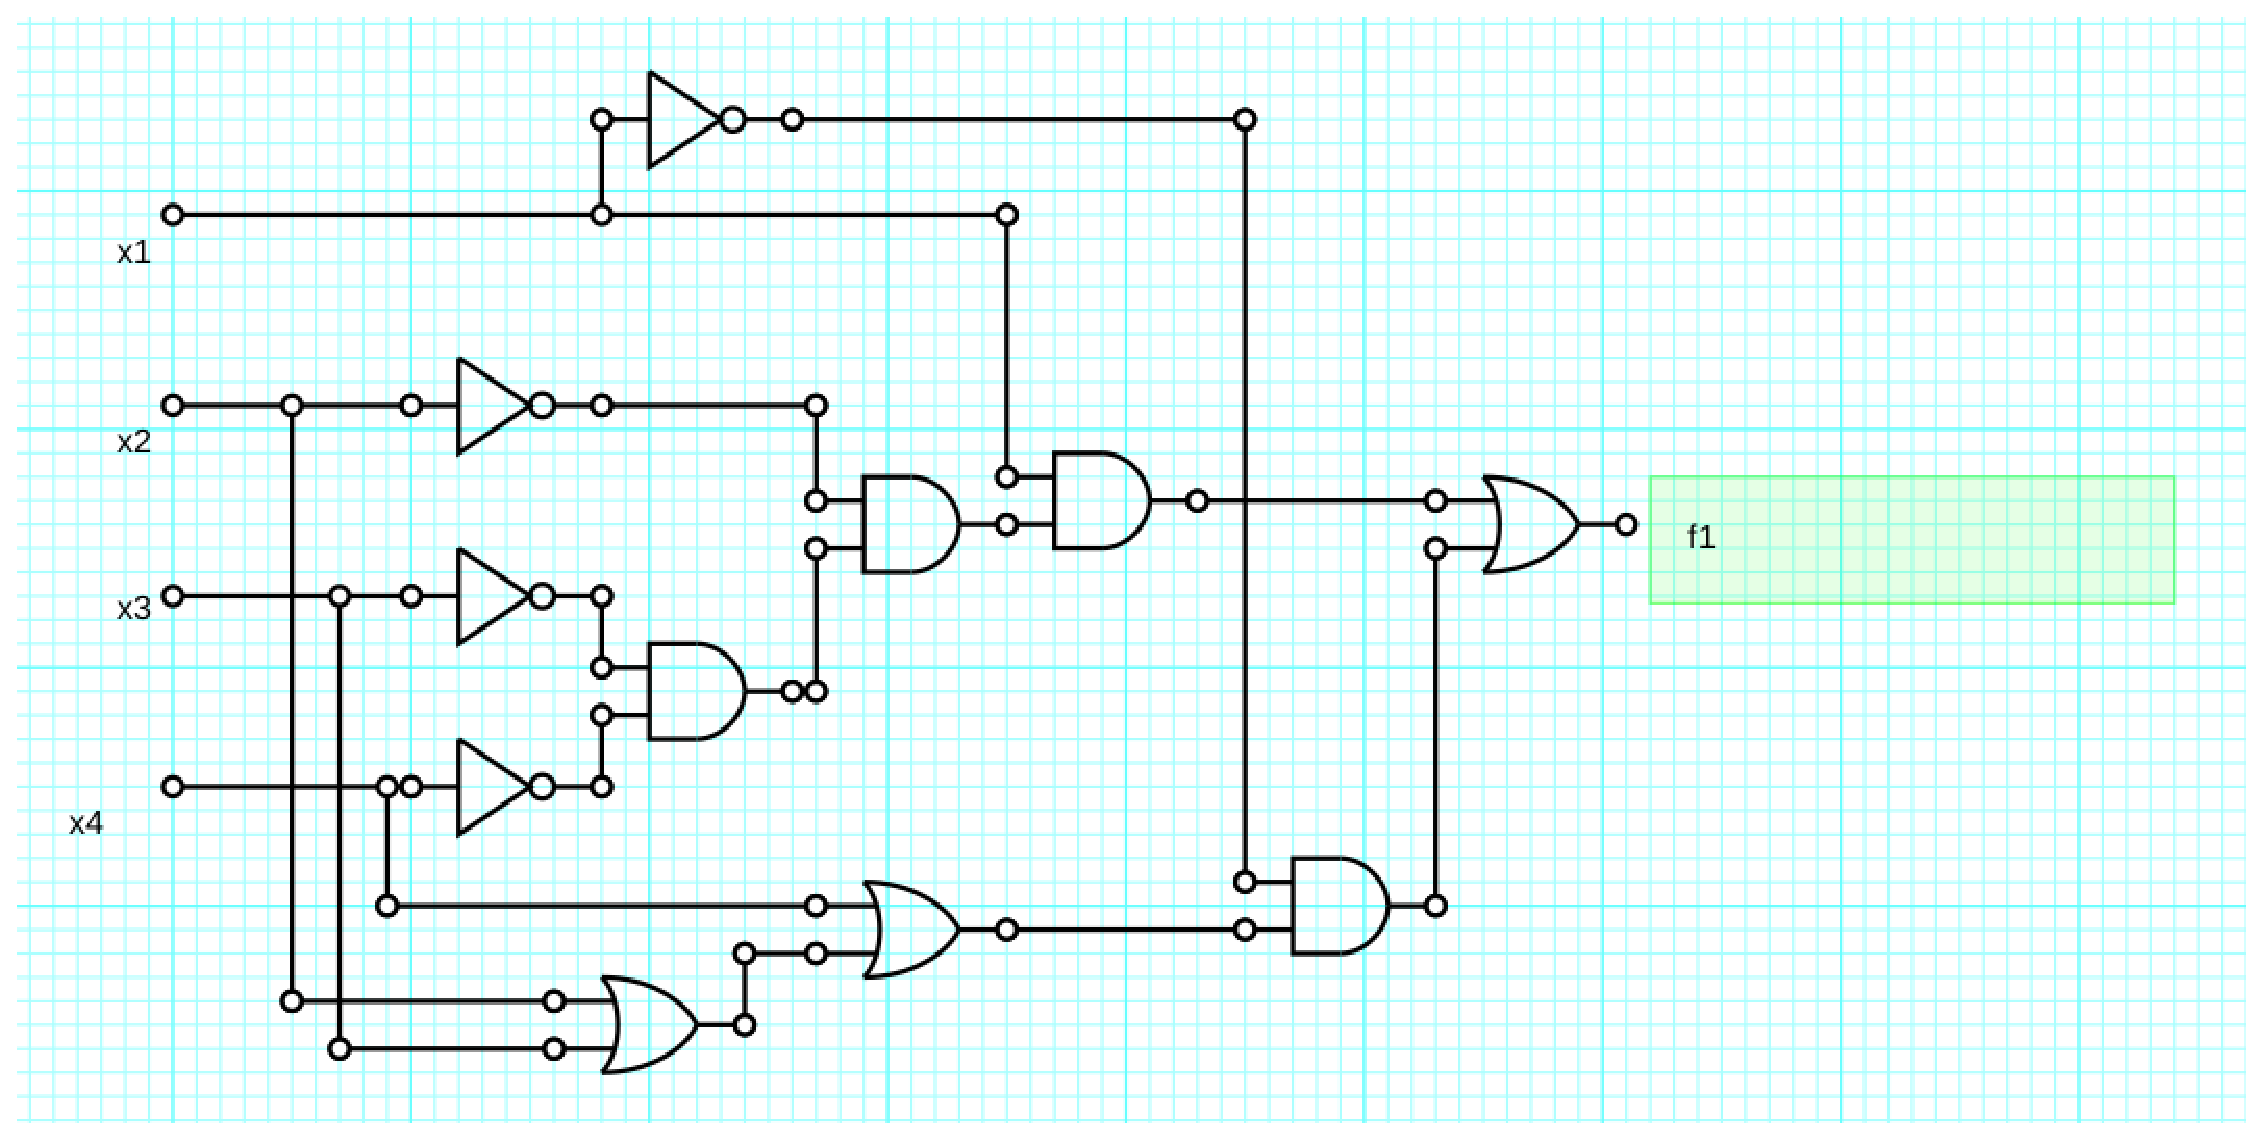
\includegraphics[scale=0.25]{E4TP1/images/1}
\par\end{centering}
\caption{\color{cyan}1st Bit's logic gates graph}
\end{figure}

\begin{figure}[!]%cambio la H por !
\begin{centering}
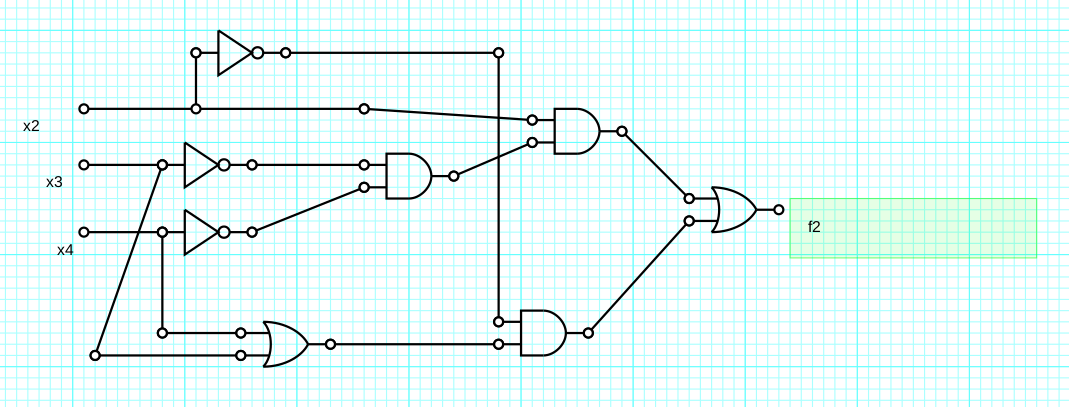
\includegraphics[scale=0.25]{E4TP1/images/2}
\par\end{centering}
\caption{\color{cyan}2nd Bit's logic gates graph}
\end{figure}

\begin{figure}[!] %cambio la H por !
\begin{centering}
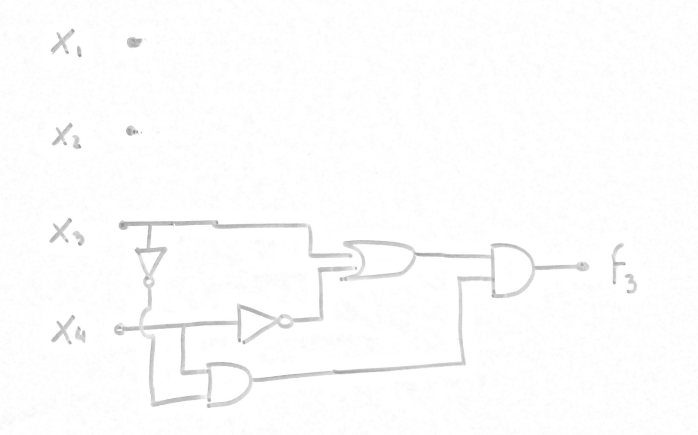
\includegraphics[scale=0.25]{E4TP1/images/3}
\par\end{centering}
\caption{\color{cyan}3rd Bit's logic gates graph}
\end{figure}

\begin{figure}[!]%cambio la H por !
\begin{centering}
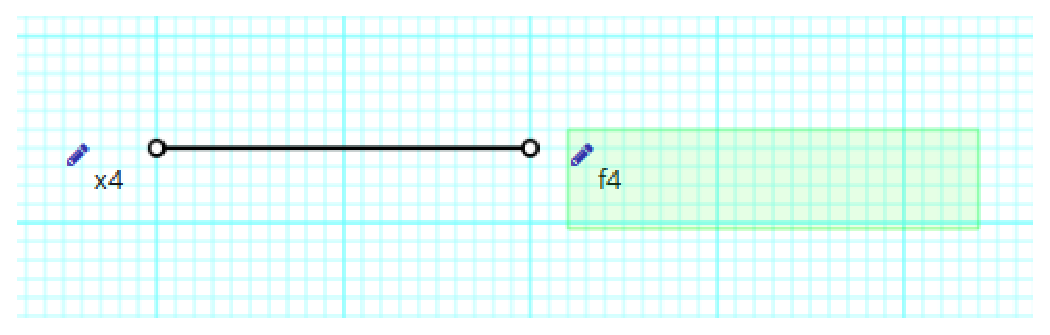
\includegraphics[scale=0.25]{E4TP1/images/4}
\par\end{centering}
\caption{\color{cyan}4th Bit's logic gates graph}
\end{figure}

Finally, this logic was implemented on verilog as follows:

\begin{figure}[!] %cambio la H por!
\begin{centering}
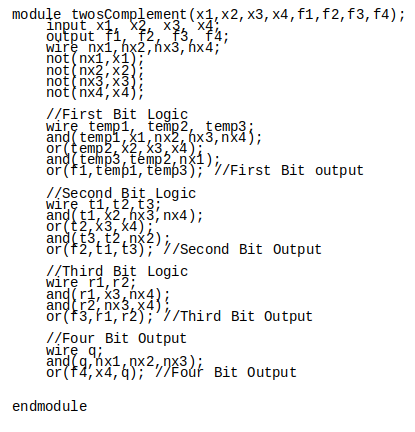
\includegraphics[scale=0.4]{E4TP1/images/5}
\par\end{centering}
\caption{\color{cyan}Verilog implementation}
\end{figure}

and, by testing the code with test.v, we have get the following output,
confirming that the code was executed correctly.

\begin{figure}[!]%cambio la H por!
\begin{centering}
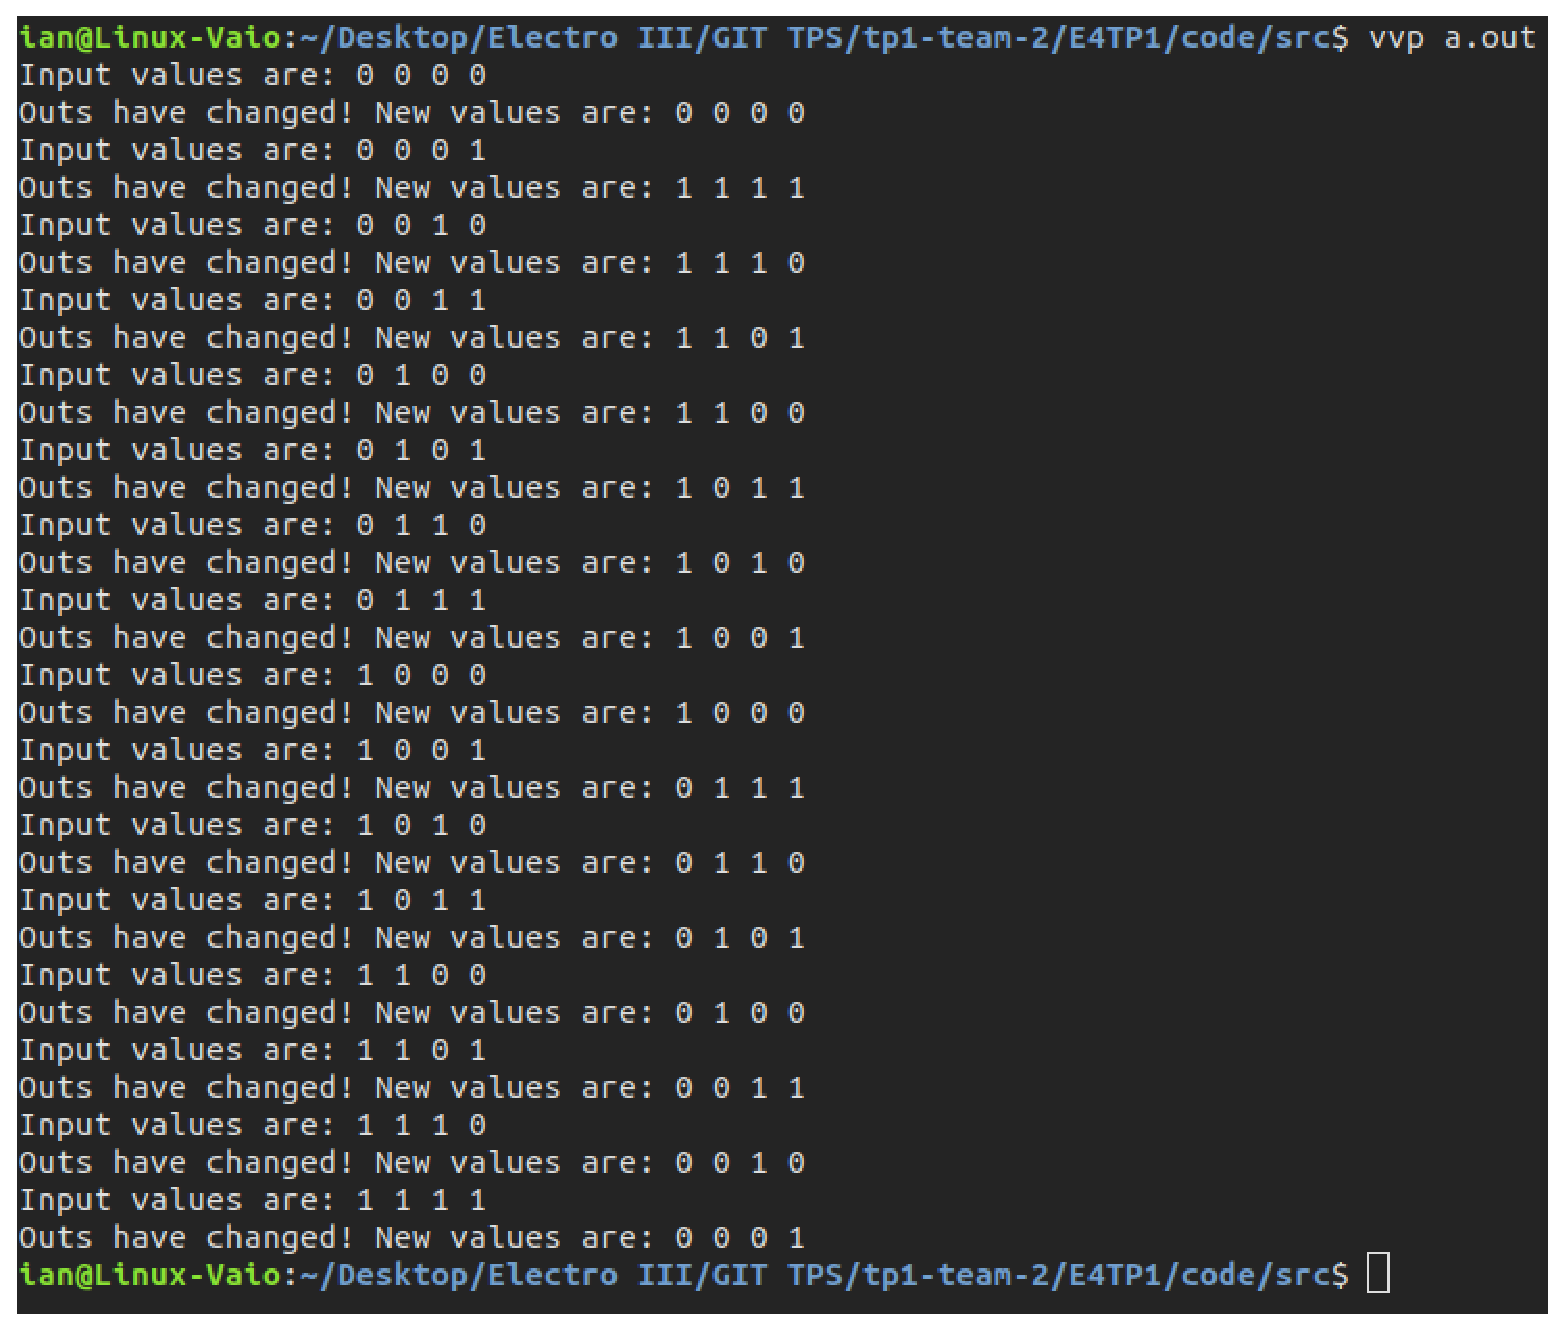
\includegraphics[scale=0.4]{E4TP1/images/6}
\par\end{centering}
\caption{\color{cyan}Terminal's output}
\end{figure}

%\end{document}
